% Template for Cogsci submission with R Markdown

% Stuff changed from original Markdown PLOS Template
\documentclass[10pt, letterpaper]{article}

\usepackage{cogsci}
\usepackage{pslatex}
\usepackage{float}
\usepackage{caption}

% amsmath package, useful for mathematical formulas
\usepackage{amsmath}

% amssymb package, useful for mathematical symbols
\usepackage{amssymb}

% hyperref package, useful for hyperlinks
\usepackage{hyperref}

% graphicx package, useful for including eps and pdf graphics
% include graphics with the command \includegraphics
\usepackage{graphicx}

% Sweave(-like)
\usepackage{fancyvrb}
\DefineVerbatimEnvironment{Sinput}{Verbatim}{fontshape=sl}
\DefineVerbatimEnvironment{Soutput}{Verbatim}{}
\DefineVerbatimEnvironment{Scode}{Verbatim}{fontshape=sl}
\newenvironment{Schunk}{}{}
\DefineVerbatimEnvironment{Code}{Verbatim}{}
\DefineVerbatimEnvironment{CodeInput}{Verbatim}{fontshape=sl}
\DefineVerbatimEnvironment{CodeOutput}{Verbatim}{}
\newenvironment{CodeChunk}{}{}

% cite package, to clean up citations in the main text. Do not remove.
\usepackage{apacite}

% KM added 1/4/18 to allow control of blind submission


\usepackage{color}

% Use doublespacing - comment out for single spacing
%\usepackage{setspace}
%\doublespacing


% % Text layout
% \topmargin 0.0cm
% \oddsidemargin 0.5cm
% \evensidemargin 0.5cm
% \textwidth 16cm
% \textheight 21cm

\title{Children's understanding of others' lexical knowledge}



\begin{document}

\maketitle

\begin{abstract}
The abstract.

\textbf{Keywords:}
communication, metalinguistics, knowledge reasoning, cognitive
development
\end{abstract}

\hypertarget{introduction}{%
\section{Introduction}\label{introduction}}

When we communicate with other people, we choose our words carefully to
transmit information that we think our partner will understand. For
instance, we referred to ``lexical'' knowledge in the title of this
paper because it conveys something precise the Cognitive Science
Conference audience. But if we were to tell a friend about the work in
this paper we would say that ``children know what words other children
probably know.''

Do you remember when you learned the word dog? What about aardvark?
While you might not be able to say the exact age at which you learned
these animals, you probably think you learned aardvark after dog. You
can probably give reasons for this intuition -- dogs are more common,
they are in lots of children's books, it's a short word, and so on.
Asked to make such judgments, adults are able to recover the order that
children actually acquire words (Kuperman, Stadthagen-Gonzalez, \&
Brysbaert, 2012). This kind of intuition could help you tune your
communication with young children, talking very differently about dogs
compared with aardvarks. Do children also have intuitions about when
words are learned? If so, these intuitions would reflect significant
metalinguistic knowledge, and may even enable them to tune their
conversation with others. In this study we ask how children infer
another's lexical knowledge, specifically whether they make item-level
predictions about what words a very young child is likely to know.

Adults show significant metalinguistic knowledge. In a large-scale
study, Kuperman, Stadthagen-Gonzalez, and Brysbaert (2012) asked adult
participants to report the age at which they understood a given word and
obtained judgments for 30,000 English words. These judgments can then be
directly compared with data on the typical age that a given word is
actually learned (also called its age of acquisition, hereafter referred
to as AoA). While adults typically overestimate the absolute age at
which they learned a given word, the estimated order in which words are
acquired is mostly intact (Kuperman et al., 2012). Adults are thus able
to make graded and surprisingly accurate relative estimates of when a
word was learned.

(if we do it in this order, do we need to make a better bridge from AoA
to what another agent knows? Like, in order for this skill to be useful
in conversation, one must be able to recruit this metalinguistic
knowledge to draw on-the-fly inferences about what an interlocutor's
likely lexical knowledge\ldots{})

From a young age, children are sensitive to their own and others'
knowledge states. As early as 12-months-old, children point more to help
an ignorant adult locate an object than a knowledgeable adult who saw
the object fall (Liszkowski, Carpenter, \& Tomasello, 2008). At age 2,
children begin to comment on, query, and discuss knowledge states
explicitly in their own language (Harris, Yang, \& Cui, 2017). By age 4,
children differentiate reliable and unreliable speakers, and privilege
information from reliable sources (e.g., Koenig \& Harris, 2005).

While a great deal of work establishes children's ability to use
situational knowledge (e.g., knowledge from perceptual access),
preschool age children have also been shown to reason about more
general, stable differences in knowledge. Preschool age children are
able to reason about expertise, for example differentiating the
knowledge of a doctor and a mechanic (Lutz \& Keil, 2002). Preschool age
children also recognize that adults typically have more linguistic
knowledge than children (Jaswal \& Neely, 2006), but also that children
might know more about some things, such as toys (VanderBorght \& Jaswal,
2008). Indeed, children are able to reason flexibly about changes in
general knowledge across development, ascribing different levels of
general knowledge to an infant, preschool child, and an adult (Fitneva,
2010; Taylor, Cartwright, \& Bowden, 1991). Beyond considering the
knowledge of specific individuals, children are also able to draw
inferences about how commonly something is known, reasoning that generic
information is likely more widely known than specific information
(Cimpian \& Scott, 2012).

Young children show an impressive ability to track other people's
knowledge across a wide range of situations, but relatively little work
has been done to probe the specificity and granularity of children's
inferences about others' knowledge. Reasoning about another person's
specific lexical knowledge may prove difficult for young children as
they also show consistent errors in reasoning about other's knowledge,
commonly over-attributing knowledge (e.g.~Gopnik \& Astington, 1988;
Taylor, Esbensen, \& Bennett, 1994). The bias to over-attribute
knowledge is particularly pronounced when the child themselves knows the
piece of information (Birch \& Bloom, 2003). After seeing inside a toy,
3-year-old children often attributed knowledge of what was inside the
toy to a puppet that had never played with the toy (Birch \& Bloom,
2003). Such curse-of-knowledge biases could severely hinder children's
ability to reason about the lexical knowledge of another child.

{[}Something about why/how we arrived at lexical knowledge as the thing
to study-- maybe the connection to communication? Bridge to our study{]}

In this study, we ask whether children have accurate estimates of other
children's knowledge. Specifically, we are interested in whether
children are sensitive to the specific vocabulary knowledge of younger
children and are able to make item-wise predictions. Such predictions
are crucial to communicate effectively with various interlocutors and
account for varying knowledge and perspectives. By age 5, children are
richly structure their language based on a listener's knowledge, for
example offering more generic information to ignorant listeners (Baer \&
Friedman, 2018). Such studies typically heavily and repeatedly emphasize
an interlocutors knowledge state, to test for children's ability to
adapt their communication in the absence of knowledge reasoning.
Children's possible difficulty specific knowledge predictions may hinder
their performance in other communication tasks (e.g.~Krauss \&
Glucksberg (1977)).

To our knowledge, only one study has asked children to give AoA
estimates for English words (Walley \& Metsala, 1992). In their study,
Walley and Metsala (1992) used a broad set of words acquired over a
large range of ages (from table to valet) to investigate young
children's general metalinguistic knowledge. As young as age 5, children
generated AoA estimates that were similar to adults'. Our study builds
on Walley and Metsala's (1992) work to collect more sensitive AoA
estimates in a single domain (animal words). To probe the specificity
and sensitivity of children's AoA estimates, the animal words we use in
this study are generally acquired within a narrow age range of 2 to 2.5,
based on parent reports of children's vocabulary (Wordbank). Our study
also differs from Walley and Metsala's (1992) in a crucial way--rather
than asking children when they themselves learned a word, we ask them to
estimate the vocabulary knowledge of another fictional child. This
framing also allowed us to not ask children the age at which they
learned a word, but instead their certainty about the other child's
knowledge. Lastly, our study also probes whether children as young as 4
might show this capacity to reason about another child's lexical
knowledge.

In the current study, children ages 4-8 were introduced to a younger
fictional child, and asked to make judgments about this fictional
child's knowledge of various animal words. We expected that overall,
children's judgments would recover the ordinal shape of age of
acquisition data for these items. That is, children would infer that the
child is most likely to know early acquired words, yielding a negative
correlation between their judgments of lexical knowledge and adult AoA
estimates. We expect developmental change in children's sensitivity to
Sam's vocabulary knowledge, with older children's judgments recovering
word-level AoA data more closely.

\hypertarget{method}{%
\section{Method}\label{method}}

\hypertarget{stimuli}{%
\paragraph{Stimuli}\label{stimuli}}

Our stimuli consisted of 15 words drawn from a single domain (animal
words), along with corresponding images of each animal. We pulled all
animal images (n = 45) from a normed image set (Rossion \& Pourtois,
2004; recoloring of Snodgrass \& Vanderwart, 1980). To ensure our
stimuli set spanned a large AoA range, we ranked the animal words from
earliest to latest AoA, using data from Kuperman et al.~(2012), and
split the words into five bins (as shown in Figure 1). In order to
select animal images that are recognizable and typically identified by a
single name, we chose the three animals from each AoA quintile with the
highest naming agreement according to a naming task with children
(Cycowicz et al., 1997). Our final stimuli consisted of these 15 items,
ordered here by estimated AoA: dog, duck, cat, pig, fish, turtle, zebra,
elephant, snake, penguin, gorilla, owl, raccoon, leopard, and lobster.
While adult AoA estimates for these words range from 2.5 to 7.5 years
old, all of these animal words are generally acquired by age 3 according
to parent reports of children's vocabulary knowledge (Wordbank?).
Because the youngest children in our study are 4 years old, we expect
all participants to know these animal words.

Participants

We pre-registered a planned sample of 60 children ages 4-8, with 12
children recruited for each year-wise age group. Due to overrecruitment,
our final sample included 65 children (12 4-year-olds, 13 5-year-olds,
13 6-year-olds, 12 7-year-olds, 15 8-year-olds). All analyses hold when
looking only at the 60 children run first chronologically. Based on our
pre-registered exclusion criterion, children who failed to answer all of
the questions were excluded and replaced (an additional 7 children).
Families were recruited online, primarily through a US University
database of families who have expressed interested in doing research or
previously participated. Children completed this study over Zoom,
interacting with a live experimenter who navigated a slide-style,
animated Qualtrics survey.

\hypertarget{procedure}{%
\subsubsection{Procedure}\label{procedure}}

\emph{Introduction.} Children were shown a picture of a fictional child
named ``Sam'' (see Figure 2). Children were anchored to Sam's knowledge
of various familiar skills, specifically some skills that Sam has
acquired (e.g., coloring), and some that Sam has not (e.g., reading).
Children are then specifically anchored to Sam's possible word knowledge
in an unrelated domain-- given an example of one word Sam knows (car),
and one word that Sam doesn't know (piano). This introduction is
intended to familiarize the children with Sam, roughly anchor them to
Sam's knowledge and age, and to ensure that children understand there
are things Sam doesn't know yet (even things children themselves likely
know, such as how to read).

\emph{General trial structure.} At each trial, children were shown a
drawing of a familiar object or animal (drawings taken from Rossion \&
Pourtois, 2004, which is a recoloring of Snodgrass \& Vanderwart, 1980).
The experimenter labelled the object for the child (e.g., ``Look, it's a
{[}ball{]}! Do you think Sam knows that this is called a {[}ball{]}? Yes
or no?''). Based on their response, children are then asked a follow-up
question: ``How sure are you that Sam {[}knows/doesn't know{]} that this
is called a {[}ball{]}-- a little sure, medium sure, or very sure?'' All
questions were presented with accompanying pictures of thumbs
{[}up/down{]} of varying size (see Figure 2). Children as young as 3 are
able to engage in uncertainty monitoring and report confidence, although
these skills do develop in the preschool years (Lyons \& Ghetti, 2011).
Children's responses to these two items were recoded onto a 1-6 scale
from 1-very sure Sam doesn't know to 6-very sure Sam knows. All trials
followed this general structure. The experimenter provided no evaluative
feedback on any trials, but did offer consistent neutral feedback (e.g.,
repeating the child's answer or saying ``Okay!''). When a child failed
to respond within about 5 seconds or offered a non-canonical response
(e.g., saying ``Maybe''), the experimenter acknowledged the child's
answer and then repeated the question with the possible responses. If a
child did not answer after the repetition was repeated, the experimenter
moved on and marked the trial as no response.

\emph{Familiarization trials.} Children first completed two non-animal
familiarization trials, one of an early-acquired word (ball) and one of
a late-acquired word (artichoke). These trials followed the trial
structure described above and were intended to help familiarize children
with the structure of the questions and scales. These trials were always
asked first and in a fixed order.

\emph{Animal trials.} Children were then shown 15 trials of the same
form for various familiar animals. For the 15 animal trials, trial order
was randomized across participants to control for any potential order
effects in children's responses.

\emph{Explanation.} After completing the final animal trial, children
were asked an open-ended explanation question about their final
judgement (e.g., ``Why do you think Sam {[}knows/doesn't know{]} that
this is called {[}an elephant{]}?'').

\emph{Final check questions.} Children were asked whether they think Sam
knows how to do two tasks: jumping and driving a car. These questions
again followed the general trial structure described above. These trials
were included as an additional check in case young children failed to
differentiate animal words based on AoA. Lastly, children were asked to
report how old they thought Sam was. This question was intended to
assess another aspect of children's belief about Sam. Sam's photo and
skill knowledge were intended to indicate toddlerhood.

\begin{CodeChunk}
\begin{figure}[tb]
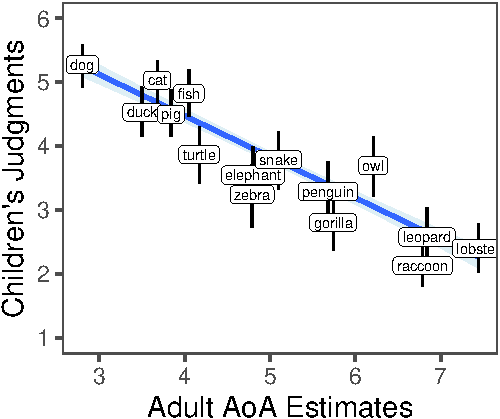
\includegraphics{figs/overall-1} \caption[Correlation between adult AoA estimates (in years, taken from Kuperman et al, 2012) and children’s judgments on our 6-point scale (1 = very sure Sam doesn’t know]{Correlation between adult AoA estimates (in years, taken from Kuperman et al, 2012) and children’s judgments on our 6-point scale (1 = very sure Sam doesn’t know; 6 = very sure Sam knows).}\label{fig:overall}
\end{figure}
\end{CodeChunk}

\hypertarget{results}{%
\section{Results}\label{results}}

Do children's judgments about a fictional character's vocabulary
knowledge reflect a sensitivity to which words are learned later? To
answer this question, we compared children's judgments on our 6-point
scale to adult judgments from Kuperman et al.~(2012). Data were analyzed
using pre-registered mixed effects model predicting children's judgments
from adult AoA estimates (Kuperman et al., 2012), including random
effects for participant and word.

First running the model without an age-term, we see a significant
negative effect of AoA on children's judgements (B = -0.67, p
\textless{} 0.001). That is, overall children judged that the fictional
child would be most likely to know an early acquired word (e.g., dog)
and least likely to know a late acquired word (e.g., lobster, see Figure
3).

\begin{CodeChunk}
\begin{figure*}[tb]
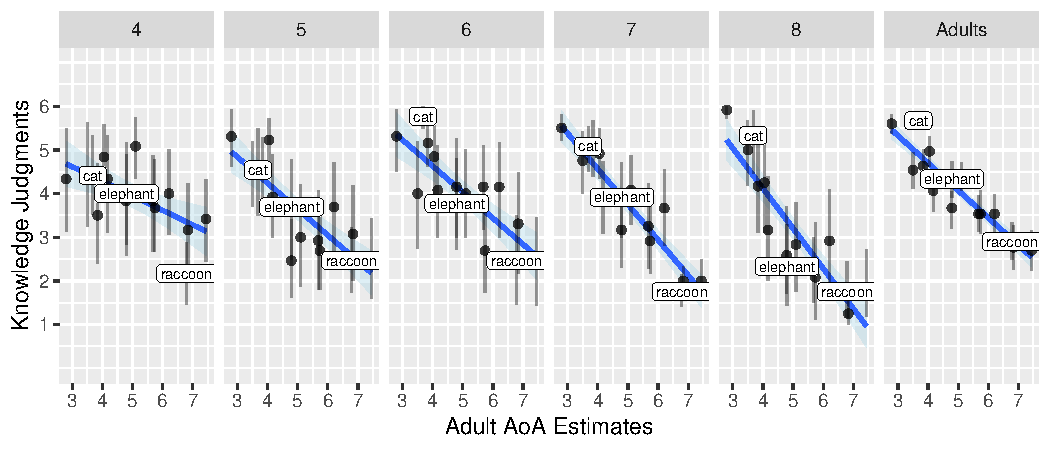
\includegraphics{figs/development-1} \caption[Children’s judgements across development]{Children’s judgements across development. Comparing adult AoA estimates (in years, taken from Kuperman et al, 2012) and children’s judgments, split by age in years.}\label{fig:development}
\end{figure*}
\end{CodeChunk}

To test for developmental changes in children's responses, we used the
same mixed effects model but included an effect of age and an
interaction between AoA and age. We expected that older children's
judgments would more closely reflect word-level AoA data, yielding a
significant interaction between AoA and child's age. That is, when
plotting children's judgments against adult AoA estimates, older
children would show steeper negative slopes than younger children.

To test the robustness of this intuition at each age, we ran the above
model separately for each group. We found a negative effect of AoA on
children's judgments at all age groups. That is, even 4-year-old
children judged that late-acquired animal words were less likely to be
known by the fictional character. We also found that the correlation
becomes more negative with children's age. {[}By age x, children's
judgments resemble those of adults{]}

\hypertarget{explanations}{%
\subsubsection{Explanations}\label{explanations}}

\hypertarget{discussion}{%
\section{Discussion}\label{discussion}}

\vspace{1em} \fbox{\parbox[b][][c]{7.3cm}{\centering Stimuli, data, and analysis code available after deanonymization.}}

\hypertarget{acknowledgements}{%
\section{Acknowledgements}\label{acknowledgements}}

This research was funded by a James S. McDonnell Foundation Scholar
Award to DY.

\hypertarget{references}{%
\section{References}\label{references}}

\setlength{\parindent}{-0.1in} 
\setlength{\leftskip}{0.125in}

\noindent

\hypertarget{refs}{}
\leavevmode\hypertarget{ref-baer2018}{}%
Baer, C., \& Friedman, O. (2018). Fitting the message to the listener:
Children selectively mention general and specific facts. \emph{Child
Development}, \emph{89}(2), 461--475.

\leavevmode\hypertarget{ref-krauss1977}{}%
Krauss, R. M., \& Glucksberg, S. (1977). Social and nonsocial speech.
\emph{Scientific American}, \emph{236}(2), 100--105.

\leavevmode\hypertarget{ref-kuperman2012}{}%
Kuperman, V., Stadthagen-Gonzalez, H., \& Brysbaert, M. (2012).
Age-of-acquisition ratings for 30,000 english words. \emph{Behavior
Research Methods}, \emph{44}(4), 978--990.

\leavevmode\hypertarget{ref-walley1992}{}%
Walley, A. C., \& Metsala, J. L. (1992). Young children's
age-of-acquisition estimates for spoken words. \emph{Memory \&
Cognition}, \emph{20}(2), 171--182.

\bibliographystyle{apacite}


\end{document}
